\documentclass{article} % For LaTeX2e
\usepackage{nips14submit_e,times}
\usepackage{amsmath}
\usepackage{amsthm}
\usepackage{amssymb}
\usepackage{mathtools}
\usepackage{hyperref}
\usepackage{url}
\usepackage{algorithm}
\usepackage[noend]{algpseudocode}
%\documentstyle[nips14submit_09,times,art10]{article} % For LaTeX 2.09

\usepackage{mathrsfs}
\usepackage{graphicx}
\usepackage{caption}
\usepackage{subcaption}

\def\eQb#1\eQe{\begin{eqnarray*}#1\end{eqnarray*}}
\def\eQnb#1\eQne{\begin{eqnarray}#1\end{eqnarray}}
\providecommand{\e}[1]{\ensuremath{\times 10^{#1}}}
\providecommand{\pb}[0]{\pagebreak}

\newcommand{\E}{\mathrm{E}}
\newcommand{\Var}{\mathrm{Var}}
\newcommand{\Cov}{\mathrm{Cov}}

\def\Qb#1\Qe{\begin{question}#1\end{question}}
\def\Sb#1\Se{\begin{solution}#1\end{solution}}

\newenvironment{claim}[1]{\par\noindent\underline{Claim:}\space#1}{}
\newtheoremstyle{quest}{\topsep}{\topsep}{}{}{\bfseries}{}{ }{\thmname{#1}\thmnote{ #3}.}
\theoremstyle{quest}
\newtheorem*{definition}{Definition}
\newtheorem*{theorem}{Theorem}
\newtheorem*{lemma}{Lemma}
\newtheorem*{question}{Question}
\newtheorem*{preposition}{Preposition}
\newtheorem*{exercise}{Exercise}
\newtheorem*{challengeproblem}{Challenge Problem}
\newtheorem*{solution}{Solution}
\newtheorem*{remark}{Remark}
\usepackage{verbatimbox}
\usepackage{listings}
\title{Linear Algebra II: \\
Problem Set IV}


\author{
Youngduck Choi \\
CIMS \\
New York University\\
\texttt{yc1104@nyu.edu} \\
}


% The \author macro works with any number of authors. There are two commands
% used to separate the names and addresses of multiple authors: \And and \AND.
%
% Using \And between authors leaves it to \LaTeX{} to determine where to break
% the lines. Using \AND forces a linebreak at that point. So, if \LaTeX{}
% puts 3 of 4 authors names on the first line, and the last on the second
% line, try using \AND instead of \And before the third author name.

\newcommand{\fix}{\marginpar{FIX}}
\newcommand{\new}{\marginpar{NEW}}

\nipsfinalcopy % Uncomment for camera-ready version

\begin{document}


\maketitle

\begin{abstract}
This work contains solutions to the problem set V
of Linear Algebra II 2016 at Courant Institute of Mathematical Sciences.
\end{abstract}

\bigskip

\begin{question}[1]
\hfill
\begin{figure}[h!]
  \centering
    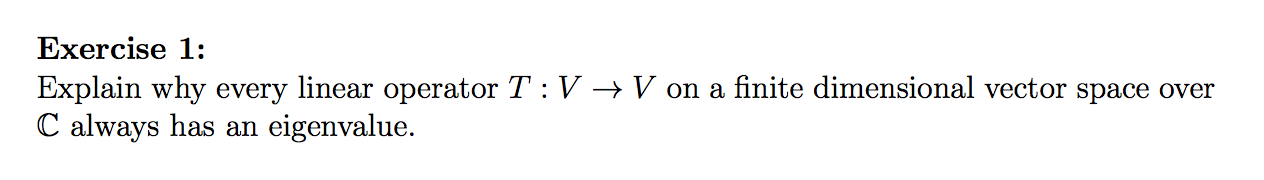
\includegraphics[width=1\textwidth]{LA-5-1.png}
\end{figure}
\end{question}
\begin{solution} \hfill \\
We know that a scalar is an eigenvalue of an operator iff it is a root to the operator's characteristic
polynomial. By the Fundemental Theorem of Algebra, we know that any polynomial over $\mathbb{C}$ splits.
Therefore, we have that any operator over $\mathbb{C}$ has an eigenvalue. 
\hfill $\qed$

\end{solution}

\bigskip

\begin{question}[2]
\hfill
\begin{figure}[h!]
  \centering
    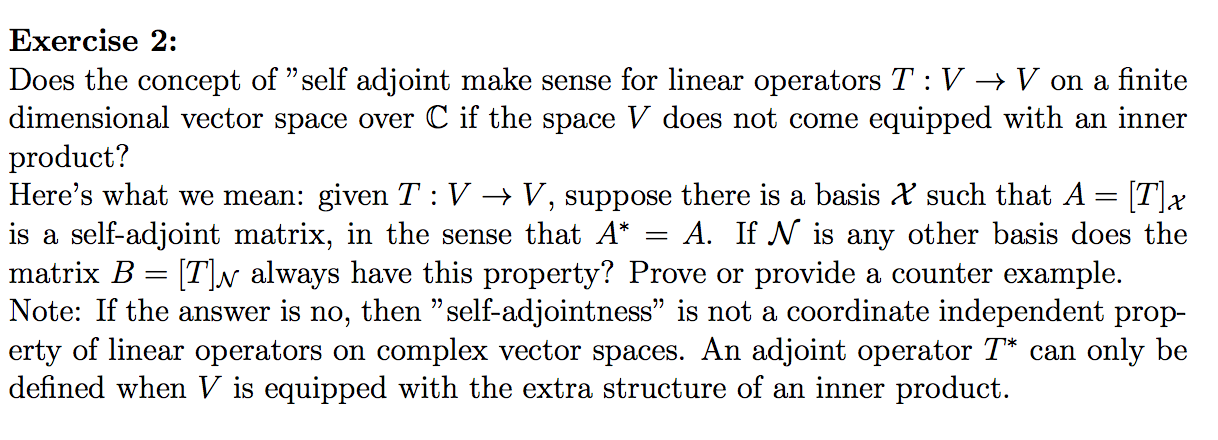
\includegraphics[width=1\textwidth]{LA-5-2.png}
\end{figure}
\end{question}
\begin{solution} \hfill \\
No. The definition of adjoint operator requires inner product structure to begin with. Therefore,
we cannot discuss whether or not an operator equals its adjoint, without the inner product structure.
As a remark, we know that the transpose of a matrix representation of a linear operator equals
the matrix representation of its adjoint, when the chosen basis is orthonormal.
\hfill $\qed$

\end{solution}

\newpage

\begin{question}[3]
\hfill
\begin{figure}[h!]
  \centering
    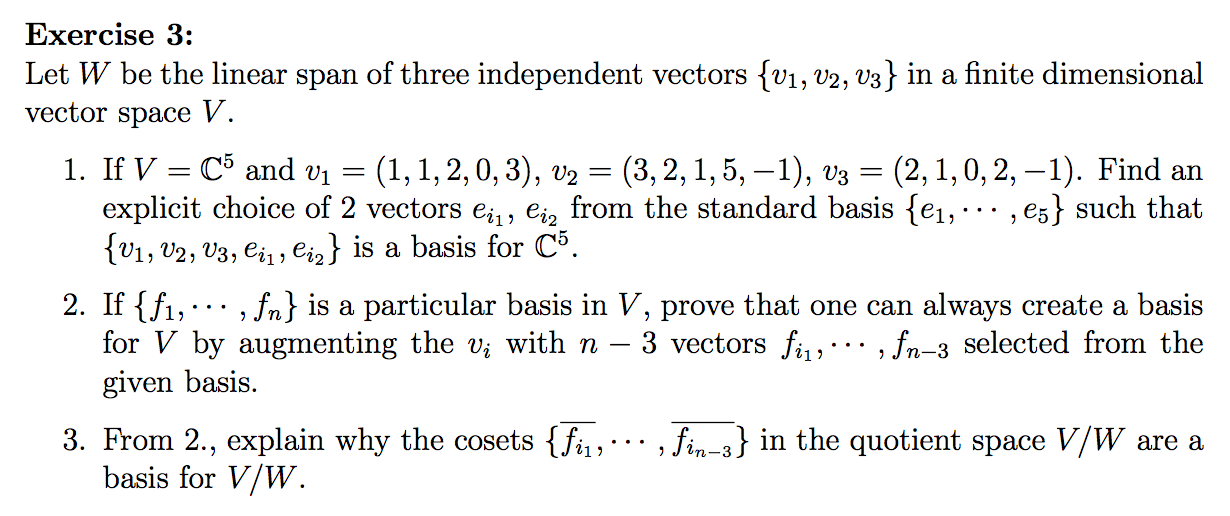
\includegraphics[width=1\textwidth]{LA-5-3.png}
\end{figure}
\end{question}
\begin{solution}
\textbf{(a)}

\bigskip

\textbf{(b)}

\bigskip 

\textbf{(c)}
As the quotient space has a dimension $\dim(V) - \dim(W)$, which can be shown using
the fundamental theorem of linear algebra and the fact that the quotient map has $W$
as the kernel, it suffices to check that the cosets are linearly independent.
Let $c_{i_1}\overline{f_{i_1}} + ... + c_{i_n}\overline{f_{i_{n-3}}} = W$. It follows that
$c_{i_1}f_{i_1} + ... + c_{i_n}f_{i_{n-3}} \in W$. Using the basis of $W$, we obtain
\eQb
c_{i_1}f_{i_1} + ... + c_{i_n}f_{i_{n-3}} &=& d_1v_1 + d_2v_2 + d_3 v_3, \\
\eQe 
which immediately gives
\eQb
c_{i_1}f_{i_1} + ... + c_{i_n}f_{i_{n-3}} - d_1v_1 - d_2v_2 - d_3 v_3 &=& 0.  \\
\eQe
By the independence of the basis set, we obtain that $c_{i_1} =...= c_{i_{n-3}} = 0$.
Therefore, the cosets form a basis of the quotient space. 

\hfill $\qed$

\end{solution}

\newpage

\begin{question}[4]
\hfill
\begin{figure}[h!]
  \centering
    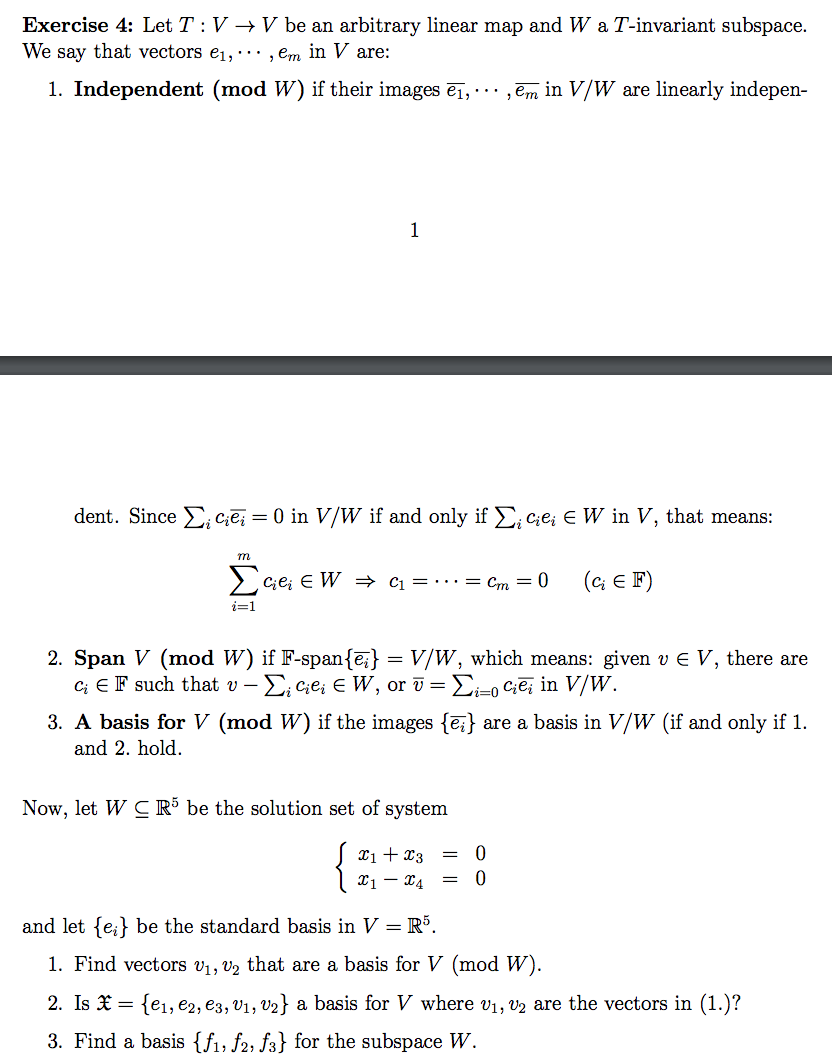
\includegraphics[width=1\textwidth]{LA-5-4.png}
\end{figure}
\end{question}
\begin{solution}

\hfill $\qed$ 
\end{solution}

\newpage

\begin{question}[5]
\hfill
\begin{figure}[h!]
  \centering
    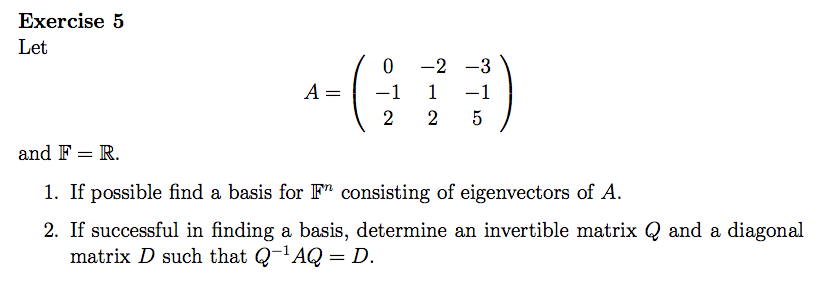
\includegraphics[width=1\textwidth]{LA-5-5.png}
\end{figure}
\end{question}
\begin{solution} \hfill \\
\textbf{(a)}
The eigenvalues are given by the roots of the following equation:
\eQb
\det  \begin{pmatrix}
-\lambda & -2 & -3 \\
-1 & 1-\lambda & -1 \\
2 & 2 & 5-\lambda \\
\end{pmatrix}  &=& 0,
\eQe
which can be simplified to 
\eQb
-(\lambda - 1)(\lambda - 2)(\lambda -3) &=& 0.
\eQe
Therefore, we have that $\lambda = 1,2,3$ are the eigenvalues of the given matrix $A$.
With the given eigenvalues, we can solve a homogenous system of equation given by $A - \lambda I = 0$
to obtain the respective eigenvectors. Doings so yields $(-1,-1,1)$, $(-1,1,0)$, and $(-1,0,1)$. 

\bigskip

\textbf{(b)} Using the information above, we have 
\eQb
Q = \begin{pmatrix}
-1 & -1 & -1 \\
-1 & 1 & 0 \\
1 & 0 & 1 \\
\end{pmatrix} \> \text{ and } \> D  = \begin{pmatrix}
1 & 0 & 0 \\
0 & 2 & 0 \\
0 & 0 & 3 \\
\end{pmatrix},
\eQe
as required.
\hfill $\qed$ 

\end{solution}


\end{document}
